\documentclass[12pt,titlepage]{article}
\usepackage{html}
\usepackage{dcolumn}
\usepackage{longtable}
\usepackage{natbib} 
\usepackage{vmargin}
\topmargin=0in
\usepackage{graphicx}
\usepackage{url}
\usepackage[reqno]{amsmath}
\usepackage{amssymb}
%\newcommand{\Amelia}{${\mathfrak{A}melia}$}
\newcommand{\Amelia}{\ensuremath{\mathfrak Amelia} }
\newcommand{\AmeliaII}{\ensuremath{\mathfrak Amelia~II} }
\usepackage{vmargin}
\topmargin=0in

\htmladdtonavigation{
  \htmladdnormallink{%
    \htmladdimg{http://gking.harvard.edu/pics/home.gif}}
  {http://gking.harvard.edu/}}
\newcommand{\hlink}{\htmladdnormallink}

\bodytext{ BACKGROUND="http://gking.harvard.edu/pics/temple.jpg"}
\setcounter{tocdepth}{3}

\title{${\mathfrak Amelia}$ II: A Program for Missing Data}

\author{James Honaker, Gary King, and Matthew Blackwell}

\begin{document}
\maketitle

\tableofcontents
\newpage



\section{Introduction}
\label{sec:intro}

This manual presents a brief introduction to the \AmeliaII software
package for multiple imputation.  James Honaker, Anne Joseph, Gary
King, Kenneth Scheve, and Naunihal Singh wrote the first version of
Amelia to remedy the discrepancy between the way social scientists
then analyzed data with missing values and the recommendations of the
statistics community.  With a few notable exceptions, statisticians
and methodologists had agreed on the advantages of the concept of
``multiple imputation'' as a general-purpose approach to data with
missing values; yet at the time most social scientists had still used
listwise deletion (deleting all observations with at least one missing
cell) or other ad hoc techniques like best guess or mean imputation to
make inferences in the presence of missing data.  These practices are
known to be inefficient and often biased.  Unfortunately, many of the
multiple imputation algorithms that had been proposed in the
literature were unfit for handling the common problems of social
science data and were often difficult to use, even for experts.

A key reason multiple imputation had not been used frequently in the
social sciences is because it was developed so that producers of large
public-use data sets could conduct the imputation for the analyst, but
this paradigm did not help those who collected, merged, or processed
their own data.  Before \citet*{KinHonJos01}, a small number of public
use data sets had been imputed, but very few researchers had imputed a
data set or used a multiply imputed data set.  The contribution of the
work that led to the first version of \Amelia was the EMis algorithm
that produced imputations requiring less expertise to use and with
more speed than existing MCMC-based algorithms.  This made it possible
to write \Amelia so that scholars could impute their own data, rather
than waiting for others to do it for them.

The \AmeliaII program goes several significant steps beyond the
capabilities of the first version of Amelia.  For one, the
boostrapping-based EMB algorithm included in \AmeliaII can impute many
more variables, with many more observations, in much less time.  The
great simplicity and power of the EMB algorithm made it possible to
write \AmeliaII so that virtually never crashes --- which to our
knowledge makes it unique among all existing multiple imputation
software.  (We have yet to find a data set that will crash \AmeliaII,
but if you find one, please let us know!)

\AmeliaII also has features to make valid and much more accurate
imputations for cross-sectional, time-series, and
time-series-cross-section data.  This software implements the ideas
developed in \citet*{HonKin06}.  Please read this paper in conjunction
with this manual.

\section{What ${\mathfrak Amelia}$ Does}
\label{sec:what}

Multiple imputation involves imputing $m$ values for each missing cell
in your data matrix and creating $m$ ``completed'' data sets.  (Across
these completed data sets, the observed values are the same, but the
missing values are filled in with different imputations that reflect
the uncertainty about the missing data.)  After imputation with
\AmeliaII's EMB algorithm, you can apply whatever statistical method
you would have used if there had been no missing values to each of the
$m$ data sets, and use a simple procedure, described in the next
paragraph, to combine the results.  (You can combine the results
automatically by doing your data analyses within Zelig, or within
Clarify for Stata; see \url{http://gking.harvard.edu/stats.shtml}.)
Under normal circumstances, you only need to impute once and can then
analyze the $m$ imputed data sets as many times and for as many
purposes as you wish.  The advantage of \AmeliaII is that it combines
the comparative speed and ease-of-use of our algorithm with the power
of multiple imputation, to let you focus on your substantive research
questions rather than spending time developing complex
application-specific models for nonresponse in each new data set.
Unless the rate of missingness is very high, $m = 5$ (the program
default) is probably adequate.

In order to combine the results across $m$ data sets, first decide on
the quantity of interest to compute, such as univariate mean,
regression coefficient, predicted probability, or first difference.
Then, the easiest way is to draw $1/m$ simulations of $q$ from each of
the $m$ data sets, combine them into one set of $m$ simulations, and
then to use the standard simulation-based methods of intepretation
common for single data sets \citep{KinTomWit00}.

Alternatively, you can combine directly and use as the multiple
imputation estimate of this parameter, $\bar{q}$, the average of the
$m$ separate estimates, $q_j$ $(j=1,...,m)$:
\begin{equation}
  \bar{q}=\frac{1}{m}\sum^{m}_{j=1}q_j.  
\end{equation}

The variance of the point estimate is the average of the estimated
variances from \emph{within} each completed data set, plus the sample
variance in the point estimates \emph{across} the data sets
(multiplied by a factor that corrects for the bias because
$m<\infty$).  Let $SE(q_j)^2$ denote the estimated variance (squared
standard error) of $q_j$ from the data set $j$, and
$S^{2}_{q}=\Sigma^{m}_{j=1}(q_j-\bar{q})^2/(m-1)$ be the sample
variance across the $m$ point estimates.  The standard error of the
multiple imputation point estimate is the square root of
\begin{equation}
SE(q)^2=\frac{1}{m}\sum^{m}_{j=1}SE(q_j)^2+S^{2}_{j}(1+1/m).
\end{equation}

Users should see especially Pp. 57-58 of \citet{KinHonJos01} for a
variety of practical suggestions in making imputations, such as what
variables to include in the imputation stage, how to keep imputations
within logically possible ranges, etc.

\section{Versions of ${\mathfrak Amelia}$}
\label{sec:versions}
Two versions of \AmeliaII are available, each with its own advantages
and drawbacks.  First, \AmeliaII exists as a package, or collection of
functions, for the R statistical software package.  Users can utilize
their knowledge of the R language to run \AmeliaII at the command line
or to create scripts that will run \AmeliaII and preserve the commands
for future use.  Alternatively, AmeliaView, an interactive Graphical
User Interface (GUI), allows users to set options and run \Amelia
without any knowledge of the R programming language.  AmeliaView
enables users to set all of the \AmeliaII options and, thus, empowers
those with limited or no coding experience to create expert level
imputations.

Both versions of \AmeliaII are available on the Windows and Linux
platforms and \AmeliaII for R runs in any environment that R can.  All
versions of ${\mathfrak Amelia}$ require the R software, which is
freely available at \url{http://www.r-project.org/}.


\section{Installation and Updates}
\label{sec:install}

Before installing \AmeliaII, you must have installed R version 2.1.0
or higher, which is freely available at
\url{http://www.r-project.org/}.
\subsection{Windows --- AmeliaView}
\label{sec:win-install}
To install AmeliaView in the Windows environment, simply download the
installer \texttt{setup.exe} from
\url{http://gking.harvard.edu/amelia/} and run it.  The installer will
ask you to choose a location to install \AmeliaII.  If you have
installed $R$ with the default options, \AmeliaII will automatically
find the location of R.  If the installer cannot find R, it will ask
you to locate the directory of the most current version of R.  Make
sure you choose the directory name that includes the version number of
R (e.g. C:/Program Files/R/R-2.2.0) and contains a subdirectory named
\texttt{bin}.  The installer will also put shortcuts on your Desktop
and Start Menu.

\subsection{Windows --- \AmeliaII for R}

Users familiar with the $R$ language, and who intend to use \Amelia
primarily as a function within other $R$ code can install all the
Amelia functions as one would install any other Amelia library.  There
is a .zip package install, which can be added to the library path.
Additionally the functions are provided in a set of five source files
which can be sourced into any $R$ code directly.  A package install can be called within R by:
  \begin{verbatim}
  > install.packages("Amelia",repos="http://gking.harvard.edu")
  \end{verbatim}
While Amelia works in builds of $R$ beyond version $2.1.0$, the online package install will only be available for the most recent version of $R$, currently, $2.3.1$. 


Even users familiar with the $R$ language may find it useful to
utilize AmeliaView to set options on variables, change arguments, or
run diagnostics.  From the command line, AmeliaView can be brought up
with the call:
  \begin{verbatim}
  > ameliagui()
  \end{verbatim}

\subsection{Linux}
\label{sec:lin-install}
To install ${\mathfrak Amelia}$ in a Linux OS, you must install the
${\mathfrak Amelia}$ library into your version of R.  This is true
even if users only wish to use AmeliaView.  Download the package from
\url{http://gking.harvard.edu/amelia}.  Then, in the same directory as
the file, at the Linux/Unix command line type
  \begin{verbatim}
  > R CMD INSTALL --library=.R/library amelia_1.0.tar.gz .
  \end{verbatim}
If you do not have access to the root, you can install the package
locally.  Create a directory (i.e. myrlibrary) to be the local storage
space for R packages.  Once this directory is created you can install
the package to that local library:
  \begin{verbatim}
  > R CMD INSTALL --library=~/myrlibrary amelia_1.0.tar.gz .
  \end{verbatim}
Once this is complete you need to edit or create your R profile.
Locate or create \texttt{~/.Rprofile} in your home directory and add
this line:
\begin{verbatim}
.libPath(``~/myrlibrary'')
\end{verbatim}
This will add your local library to the list of library paths that R
searches in when you load libraries.

Linux users can use AmeliaView in the same way as Windows users of
\Amelia for R.  From the command line, AmeliaView can be brought up
with the call:
  \begin{verbatim}
  > AmeliaView()
  \end{verbatim}

\section{Program Overview}
\label{sec:overview}

\subsection{AmeliaView}
\label{sec:guioverview}
Built around the core of the R library, AmeliaView has a graphic
interface for users to input data, set options, create the imputed
data sets, and run diagnostics.  The structure of the program moves
logically through these steps.  In Windows, this can be accessed from
the desktop shortcut created by the installer.  In Linux, accessing
the GUI requires calling a function from within R\footnote{AmeliaView
  can be called from within R in Windows, as well, using the
  \texttt{AmeliaView()} function.}.  Once AmeliaView is open, no direct
use of R is required.

The main window of AmeliaView is divided into three steps.  In Step 1,
you indicate the location of your data and load it into the program.
In Step 2, you can set options about your data by using the Options
dialogs.  In Step 3, you can set options about the output of
${\mathfrak Amelia}$ and execute the ${\mathfrak Amelia}$ code.  You
have the option to save your output data files for further use.

In most simple applications, all you will need to do is load an input
data file, set any options you desire, and hit the ``Run Amelia''
button.  For example:
\begin{enumerate}
\item Specify the type of data file you wish to input by using the
  ``Input Data Type'' drop-down menu.  Next, use the ``Browse...''
  button to find the location of your data file.  Once this is
  specified, you can hit the ``Load Data'' button to load the data.
  If your data loads correctly, the status bar at the bottom of the
  program will show the filename, number of rows and number of
  columns.  At this point you can use the ``Summarize Data'' button to
  view summary statistics about the variables along with histogram
  plots of them.
\item In the Options step, you can specify the time series and cross
  sectional variables in your data set (if any) by using the
  appropriate drop-down menus.  Each of the ``Variables'', ``TSCS'',
  and ``Priors'' buttons open a separate dialog box in which you can
  set options in each of these categories.
\item In the Output step, you can specify what file type (if any) in
  which you would like to save your output data.  You can also set the
  name of the output data and the number of data sets you would like.
  You can now run ${\mathfrak Amelia}$ by pressing the ``Run Amelia''
  button.  A dialog will open that tracks the progress of ${\mathfrak
    Amelia}$ and will let you know when it has finished.  Once this is
  complete, you can either use the diagnostics or close ${\mathfrak
    Amelia}$.
\end{enumerate}

\ 
\subsection{\Amelia for R}

\label{sec:roverview}
Using \Amelia in $R$ you will first have to load the library into R
using the \texttt{library(Amelia)} command.  Once the package is
loaded, you can set options using the arguments of the
\texttt{amelia()} function.  The output data will be either a list of
$m$ data frames or matrices depending on your input data.  Please
refer to the end of this manual for detailed documentation on
adjusting the optional arguments from their default values.

\section{Data Input and Output}
\label{sec:data}

\subsection{AmeliaView}
\label{sec:data-gui}
AmeliaView uses the ``foreign'' package in R to import and export
various types of files.  In the Input box, you can choose the file
type you wish to use from the group of supported file types: Comma
Separated Values (.csv), Tab-Delimited (.txt), Stata (.dta), SPSS
(.dat), and SAS Transport (.xport). Once this is set, you can proceed
to locate your file in one of two ways.  You can type the location of
the file in the ``Input Data File'' entry and press the ``Load Data''
button.  Or you can locate your file by using the ``Browse...'' button
to select the file of your choice.  Once you have entered the file
name, press the ``Load Data'' button to load the file into ${\mathfrak
  Amelia}$.

When you have loaded the data, you can use the ``Summarize Data''
button to see the data.  This includes seeing the minimum and maximum
values along with the mean and standard deviation.  Another feature is
the ability to view a plot of the histogram of each individual
variable.  This can help you get a graphical sense of the observed
values in your dataset.

Fewer options exist for the output data files due to the limitations
of the ``foreign'' package.  You can only save the imputed datasets as
either a CSV, Tab-Delimited, or Stata file. However, most statistical
packages will allow you to read in datasets as either CSV or
Tab-delimited.  The names of the files will be the name you specify,
plus a number appended at the end to distinguish between successive
imputed datasets.  For example, if you set the name to be ``mydata''
and the output file type to be CSV, your files would be:
\begin{verbatim}
mydata1.csv
mydata2.csv
...
\end{verbatim}
There will be as many datasets as you indicate in the output options
box.

Another output file that is produced when running ${\mathfrak Amelia}$
is the Replication Archive.  This file can be used to reproduce the
same set of options you ran ${\mathfrak Amelia}$ with so that you or
anyone else can replicate the same findings.  This file automatically
saves to ``amarchive.r''.  (If, as is becoming standard practice, you
create and archive replication data sets to accompany your papers
\citep{King95}, you should include this file.)This file can also serve
as a session save that can be opened later to load the same options
that you ran ${\mathfrak Amelia}$ under.  This allows you to pick up
where you left off in the next run of ${\mathfrak Amelia}$, adjust
options and rerun the imputations, or return at a later point and use
the diagnostic routines.

\subsection{\Amelia for R}
\label{sec:data-r}
Data input in the command-line version of ${\mathfrak Amelia}$ for R
is identical to any data input in R.  You must have your data in
either a text format such as Comma Separated Values (.csv) or
Tab-Delimited (.txt) and then read them into R (generally this would
involve the functions \texttt{read.csv} or \texttt{read.table},
respectively).  You can read about the specifics of how to load data
into R in the R documentation or in Zelig
(\url{http://gking.harvard.edu/zelig}).  Of course your data may be
generated by code and amelia called as a function later in that code.

Besides various commercial packages to transfer your data between
formats, a viable option is using the \texttt{foreign} package.  This
package can greatly expand the number of different formats that R can
input, including Stata, SPSS, and SAS transport.

Whichever way you get your data into R, when passing it to the
\texttt{amelia} function, it can either be in the form of a data frame
or matrix.  After ${\mathfrak Amelia}$ has run, you will get datasets
returned in the same type as the format of the dataset given to the
amelia function.  Once you have these datasets, you can manipulate
them in R or save them to files using the R function \texttt{write}.

For example, a simple session or code fragment might be:
  \begin{verbatim}
  > library(amelia)
  > x<-read.table("mydata.csv")
  > output<-amelia(data=x,empri=10,amords=c(3,4))
  > save(output,file="output.rData")
  \end{verbatim}
where \texttt{amords} and \texttt{empri} are options detailed later in
this manual.

\section{Options}
\label{sec:options}
There are a variety of options in \Amelia that customize the
imputation model to handle problems that are common in social science
data.  In AmeliaView, these options are set using the dialog boxes
``Variables,'' ``TSCS,'' and ``Priors.''  At these dialogs, the user
can visually inspect and set each option.  Please refer to the Menu
Guide below for details on the content of the dialogs.

In \Amelia for R, these options must be set on the command line.  From
within R, users can set the transformations by including a vector of
column numbers or names (if column names exist), that \Amelia should
transform.  For example,

\begin{verbatim}
> amelia(mydata, noms=c(2,3,7))
\end{verbatim}
or
\begin{verbatim}
> amelia(mydata, logs=c(``gdp'',``population''))
\end{verbatim}

\subsection{Screen Output}
The output of the imputation model in the AmeliaView program appears
in a new window.  It lists stages of the imputation model, including
the number of iterations of the EM chain necessary in each of the
bootstraps.

Screen output in the $R$ command level can be adjusted with the
``print to screen'' argument, \texttt{p2s}.  At a value of 0, no
screen printing will occur.  This may be useful in large jobs or
simulations where a very large number of imputation models may be
required.  The default value of 1, lists each bootstrap, and displays
the number of iterations required to reach convergence in that
bootstrapped dataset.  The value of 2 gives more thorough screen
output, including, at each iteration, the number of parameters that
have significantly changed since the last iteration.  This may be
useful when the EM chain length is very long, as it can provide an
intuition for many parameters still need to converge in the EM chain,
and a sense of the time remaining.  However, it is worth noting that
the last several parameters can often take a significant fraction of
the total number of iterations to converge.

\subsection{Transformations of Variables}
\label{sec:trans}

Social science data commonly includes variables that fail to fit into
a multivariate normal distribution. Indeed, numerous models have been
introduced specifically to deal with the problems they present.  As it
turns out, much evidence in the literature (discussed in
\citealt{KinHonJos01}) indicates that the multivariate normal model
used in ${\mathfrak Amelia}$ usually works well for the imputation
stage even when discrete or non-normal variables are included and when
the analysis stage involves these limited dependent variable models.
Nevertheless, ${\mathfrak Amelia}$ includes some limited capacity to
deal directly with ordinal and nominal variables and to variables that
require other transformations.  In general nominal and log transform
variables must be declared to \Amelia, whereas ordinal (including
dichotomous) variables often need not be, as described below.  (For
harder cases, see Schafer, 1997, for specialized MCMC-based imputation
models for discrete variables.)\nocite{KinHonJos01}

Although these transformations are taken internally on these variables
to better fit the data to the multivariate normal assumptions of the
imputation model, all the imputations that are created will be
returned in the original untransformed form of the data (If the user has \emph{already} performed transformations on their data (such as taking a log or square root) these do not need to be declared, as that would result in the transformation occuring \emph{doubly} in the imputation model).  The fully
imputed datasets that are returned will always be in the form of the
original data that is passed to the amelia routine.

\subsubsection{Ordinal}
\label{sec:ord}
In much statistical research, researchers treat independent ordinal
(including dichotomous) variables as if they were really continuous.
If the analysis model to be employed is of this type, then nothing
extra is required of the of the imputation model. Users are advised to
allow ${\mathfrak Amelia}$ to impute non-integer values for any
missing data, and to use these non-integer values in their analysis.
Sometimes this makes sense, and sometimes this defies intuition. One
particular imputation of 2.35 for a missing value on a seven point
scale carries the intuition that the respondent is between a 2 and a 3
and most probably would have responded 2 had the data been observed.
This is easier to accept than an imputation of 0.79 for a dichotomous
variable where a zero represents a male and a one represents a female
respondent. However, in both cases the non-integer imputations carry
more information about the underlying distribution than would be
carried if we were to force the imputations to be integers. Thus
whenever the analysis model permits, missing ordinal observations
should be allowed to take on continuously valued imputations.

Often, however, analysis models require some variables to be strictly
ordinal, as for example the dependent variable must be in a logistical
regression.  Imputations for variables set as ordinal are created by
taking the continuously valued imputation and using an appropriately
scaled version of this as the probability of success in a binomial
distribution. The draw from this binomial distribution is then
translated back into one of the ordinal categories.

\subsubsection{Nominal}
\label{sec:nom}
Nominal variables (other than dichotomous) must be treated quite
differently than ordinal variables. Any multinomial variables in the
data set (such as religion coded 1 for Catholic, 2 for Jewish, and 3
for Protestant) must be specified to ${\mathfrak Amelia}$.

For a $ p$-category multinomial variable, ${\mathfrak Amelia}$ will
determine $ p$ (as long as your data contain at least one value in each
category), and substitute $ p-1$ binary variables to specify each
possible category. These new $ p-1$ variables will be treated as the
other variables in the multivariate normal imputation method chosen,
and receive continuous imputations. These continuously valued
imputations will then be appropriately scaled into probabilities for
each of the $ p$ possible categories, and one of these categories will
be drawn, where upon the original $ p$-category multinomial variable
will be reconstructed and returned to the user. Thus all imputations
will be appropriately multinomial.

Since ${\mathfrak Amelia}$ properly treats a $ p$-category multinomial
variable as $ p-1$ variables, one should understand the number of
parameters that are quickly accumulating if many multinomial variables
are being used. If the square of the number of real and constructed
variables is large relative to the number of observations, the user is
recommended to implement a ridge prior distribution on the parameter
space.

\subsubsection{Natural Log}
\label{sec:log}
If one of your variables is heavily skewed or has outliers that may
alter the imputation in an unwanted way, you can use a natural
logarithm transformation of that variable in order to normalize its
distribution.  This transformed distribution helps ${\mathfrak Amelia}$
to avoid imputing values that depend too heavily on outlying data
points.  Log transformations are common in expenditure and economic
variables where we have strong beliefs that the marginal relationship
between two variables decreases as we move across the range.

\subsubsection{Square Root}
\label{sec:sqrt}
Event count data is often heavily skewed and has nonlinear
relationships with other variables.  One common transformation to
tailor the linear model to count data is to take the square roots of
the counts.  This is a transformation that can be set as an option in
amelia.
 
\subsubsection{Logistic}
\label{sec:lgstc}
Proportional data is sharply bounded between 0 and 1.  A logistic
transformation is one possible option in amelia to make the
distribution symmetric and relatively unbounded.

\subsection{Identification Variables}
\label{sec:idvars}
Datasets often contain identification variables, such as country
names, respondent numbers, or other id numbers, codes or
abbreviations.  Sometimes these are text and sometimes these are
numeric.  Often it is not appropriate to include these variables in
the imputation model, but it is useful to have them remain in the
imputed datasets (However, there are models that would include the ID
variables in the imputation model, such as fixed effects model for
data with repeated observations of the same countries).
Identification variables which are not to be included in the
imputation model can be identified with the argument \texttt{idvars}.
These variables will not be used in the imputation model, but will be
kept in the imputed datasets.

In order to conserve memory, it is wise to remove unnecessary
variables from a data set before loading it into ${\mathfrak Amelia}$.
The only variables you should include in your data when running
${\mathfrak Amelia}$ are variables you will use in the analysis stage
and those variables that will help in the imputation model.  While it
may be tempting to simply mark unneeded variables as IDs, it only
serves to waste memory and slow down the imputation procedure.

\subsection{Time Series, or Time Series Cross Sectional Data} \label{sec:tscs}

Many variables that are recorded over time within a cross-sectional
unit are observed to vary smoothly over time.  In such cases, knowing
the observed values of observations close in time to any missing value
may enormously aid the imputation of that value.  However, the exact
pattern may vary over time within any cross-section.  There may be
periods of growth, stability, or decline; in each of which the
observed values would be used in a different fashion to impute missing
values.  Also, these patterns may vary enormously across different
cross-sections, or may exist in some and not others.  ${\mathfrak
  Amelia}$ can build a general model of patterns within variables
across time by creating a sequence of polynomials of the time index.
If, for example, $GDP$ varies smoothly over time, then we make the
modeling assumption that there exists some polynomial that describes
the economy in cross-sectional unit $i$ at time $t$ as:
\begin{equation}
\textrm{GDP}(t)_i = \beta_0 + \beta_1 t + \beta_1 t^2 + \beta_1 t^3 \ldots
\end{equation}
And thus if we include enough higher order terms of time then the
pattern between observed values of GDP can be estimated.  ${\mathfrak
  Amelia}$ will create polynomials of time up to the user defined
$k$-th order, ($k\leq3$).  If cross-sectional units are specified
these polynomials can be interacted with the cross-section unit (this
is the default) to allow the patterns over time to vary between
cross-sectional units.  Unless you strongly believe all units have the
same patterns over time in all variables (including the same constant term), this is a reasonable
default.  When $k$ is set to 0, this interaction simply results in a
model of \emph{fixed effects} where every unit has a uniquely
estimated constant term.  \AmeliaII does not smooth the observed data,
and only uses this functional form, or one you choose, with all the
other variables in the analysis and the uncertainty of the prediction,
to impute the missing values.

In AmeliaView, the TSCS settings can be adjusted in the Time Series
Cross-Sectional Dialog (discussed in section \ref{sec:tscsdiag} of
this manual).  At the $R$ command line, these options can be set as:

\begin{verbatim}
> amelia(mydata, ts=1, cs=2, polytime=2, intercs=TRUE)
\end{verbatim} 

Where \texttt{ts} and \texttt{cs} give the locations of the time and
cross-section indicators (often country names and years,
respectively), \texttt{polytime} is an integer between 0 and 3
inclusive, that sets the order of polynomials to use, and
\texttt{intercs} defines whether these polynomials should be
interacted with the cross-sectional unit.

\section{Setting Priors} \label{sec:obspri}

${\mathfrak Amelia}$ has a number of methods of setting priors within
the imputation model.  Two of these are commonly used and discussed
below, empirical or ridge priors and observational priors.

\subsection{Empirical (Ridge) Priors for High Missingness, 
  Small \emph{n}'s, or Large Correlations}\label{sec:prior}

When the data to be analyzed contain a high degree of missingness or
very strong correlations among the variables, or when the number of
observations is only slightly greater than the number of parameters
$p(p+3)/2$ (where $p$ is the number of variables), results from your
analysis model will be more dependent on the choice of imputation
model.  This suggests more testing in these cases of alternative
specifications under ${\mathfrak Amelia}$.

In these circumstances, we recommend adding a ridge prior which will
help with numerical stability by shrinking the covariances among the
variables toward zero without changing the means or variances.  The
ridge prior can be implemented by setting the option \texttt{empri} in
R and the Ridge Prior entry under the ``Priors'' button in the
standalone.  Including this prior as a positive number is roughly
equivalent to adding \texttt{empri} artificial observations to the
data set with the same means and variances as the existing data but
with zero covariances.  Thus, increasing the \texttt{empri} setting
results in more shrinkage of the covariances, thus putting more a
priori structure on the estimation problem: like many Bayesian
methods, it reduces variance in return for an increase in bias that
one hopes does not overwhelm the advantages in efficiency.  In
general, we suggest keeping the value on this prior relatively small
and increase it only when necessary.  A recommendation of 0.5 to 1
percent of the number of observations, $n$, is a reasonable starting
value, and often useful in large datasets to add some numerical
stability.  For example, in a dataset of two thousand observations,
this would translate to a prior value of 10 or 20 respectively.  A
prior of up to 5 percent is moderate in most applications.

\subsection{Observation-level priors}
\label{sec:obspri}

Reseachers often have additional prior information about missing data 
values based on previous research, academic consensus, or personal 
experience.  Amelia can incorporate this information to produce vastly 
improved imputations.  The Amelia algorithm allows users to include 
informative Bayesian priors about individual missing data cells 
instead of the more general model parameters, many of which have 
little direct meaning.  

The incorporation of priors follows basic Bayesian analysis where the 
imputation turns out to be a weighted average of the model-based 
imputation and the prior mean, where the weights are functions of the 
relative strength of the data and prior: when the model predicts very 
well, the imputation will downweight the prior, and vice versa.  

The priors about individual observations should describe the analyst's 
belief about the distribution of the missing data cell.  This can either 
take the form of a mean and a standard deviation or a confidence interval.  For instance, we 
might know that GDP growth for Ghana in a given year was somwhere 
around $3.5\%$, but we have some uncertainty as to the exact value.   
Our prior belief about the distribution of the missing data cell, then, 
centers on $3.5$ with a standard deviation that reflects the amount of 
uncertainty we have about our prior belief. 

In AmeliaView, the observational priors dialog will guide you through 
adding priors to the imputation.  Refer to section \ref{sec:refobspri} for 
further details on how to add priors in AmeliaView.

Alternatively, in R, you must build two matrices, one for the mean and
one for the standard deviation, both of which have the same
dimensions as the original data matrix.  To add the prior, first note
the cell position of the missing data value in question; that is, find
its row and column number in R.  From here, find the same position in
the matrix of prior means and place your prior belief about the mean
in this cell.  Repeat the same procedure for the standard deviation
and then include them with the \texttt{amelia} function with the
\texttt{means} and \texttt{sds} arguments.  An example of this would
go as follows:

\begin{verbatim}
 > n <- nrow(data)  ## grab the rows of the data
 > p <- ncol(data)  ## grab the columns of the data
 > means.priors <- matrix(NA,nrow=n,ncol=p)  ## make priors matrices of
 > sds.priors <- matrix(NA,nrow=n,ncol=p)  ## the same size as the data
 > means.priors[150,4] <- 3.5
 > sds.priors[150,4] <- .5  ## set priors for the cell at row 150, column 4
 > amelia.out <- amelia(data = data, means = means.priors, sds = sds.priors)
\end{verbatim}


\section{Diagnostics}\label{sec:diag}

\Amelia currently provides three diagnostic tools to inspect the
imputations that are created.  These routines \texttt{compare},
\texttt{overimpute} and \texttt{overdisperse} graphically investigate

the distribution of the imputations, the fit of the imputation model,
and modality of the Likelihood space optimized by the EM chain,
respectively.

\subsection{Compare}

In the diagnostic window of AmeliaView, the compare function will, for
a given variable, generate a plot of the relative frequencies of the
observed data with an overlay of the relative frequency of the imputed
values.  The imputed curve plots the density of the \emph{mean}
imputation over the $m$ datasets.  That is, for each cell that is
missing in the variable the diagnostic will find the mean of that
cell in each of the $m$ datasets and use that value for the density
plot.  These graphs will allow you to inspect how the density of
imputations compares to the density of observed data. Some discussion
of these graphs can be found in \citet*{AbaGelLev05}.  Minimally, these
graphs can be used to check that the mean imputation falls within
known bounds, when such bounds exist in certain variables or settings.
\begin{figure}[htp!]
  \centering 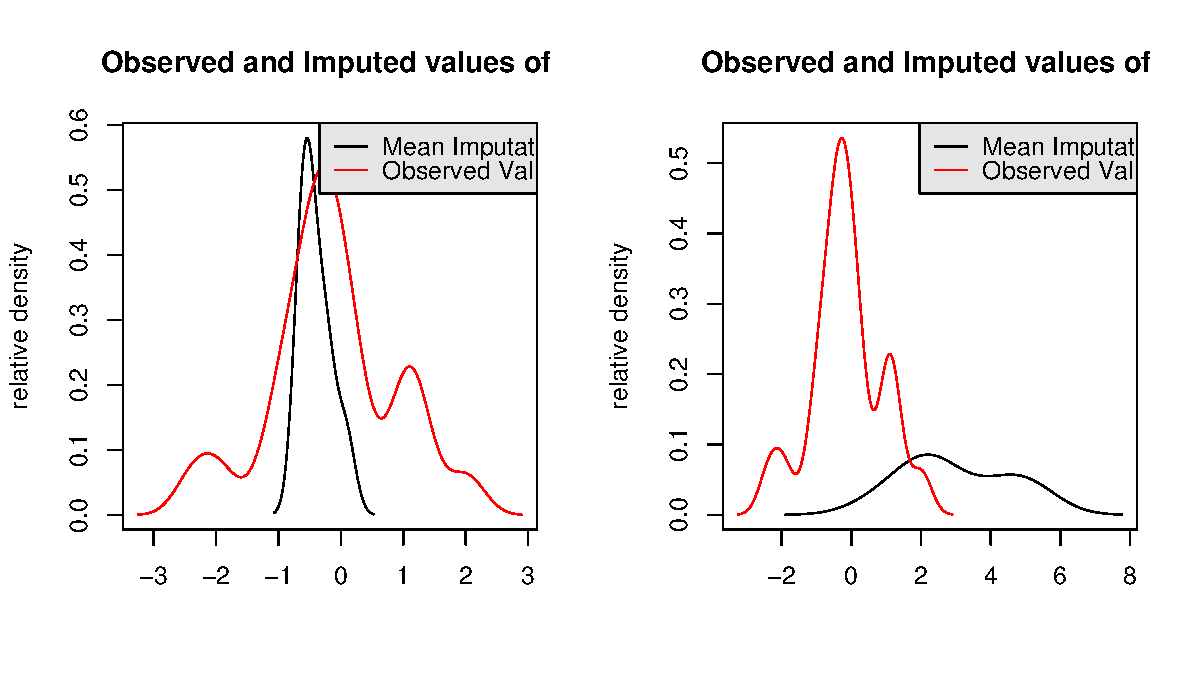
\includegraphics[scale=.8]{comp}
  \caption{Two examples of the compare diagnostic graph.  In the left
    graph all the imputations, the density of which is shown in black,
    are contained within the range of the observed data for this
    variable (in red).  In the right graph some of the mean imputed
    values are larger than the largest observed value.  This may be
    reasonable (if for example, high income respondents to a survey do
    not report their income) or may be a warning to change the
    imputation model, if for example the data has strong bounds and
    these imputations fall well outside these bounds.}
  \label{f:oi1}
\end{figure}


This graph can also be called from $R$ as:
\begin{verbatim}
 > output<-amelia(data=x) 
 > compare.density(data=x,output=output,var=3)
\end{verbatim}
where \texttt{var} is the column number (or the name) of the variable
you would like to produce the graph for.

\subsection{Overimpute}
\label{sec:overimpute}

\emph{Overimputing} is a technique we have developed to judge the fit
of the imputation model.  Because of the nature of the missing data
mechanism, it is impossible to tell whether the mean prediction of the
imputation model is close to the unobserved value that is trying to be
recovered.  By definition this missing data does not exist to create
this comparison, and if it existed we would no longer need the
imputations or care about their accuracy.  However, a natural question
the applied researcher will often ask is how accurate are these
imputed values?

Overimputing involves sequentially treating each of the
\emph{observed} values as if they had actually been missing.  For each
observed value in turn we then generate several hundred imputed values
of that observed value, \emph{as if it had been missing}.  While $m=5$
imputations are sufficient for most analysis models, this large number
of imputations allows us to construct a confidence interval of what
the imputed value would have been, had any of the observed data been
missing.  We can then graphically inspect whether our observed data
tends to fall within the region where it would have been imputed had
it been missing.

Our overimputation diagnostic runs this procedure through all of the
observed values for a user selected variable.  We can graph the
estimates of each observation against the true values of the
observation.  On this graph, a $y=x$ line indicates the line of
perfect agreement; that is, if the imputation model was a perfect
predictor of the true value, all the imputations would fall on this
line.  For each observation, \Amelia also plots 90\% confidence
intervals that allows the user to visually inspect the behavior of the
imputation model. By checking how many of the confidence intervals
cover the $y=x$ line, we can tell how often the imputation model can
confidently predict the true value of the observation.

\begin{figure}[htp!]
  \centering 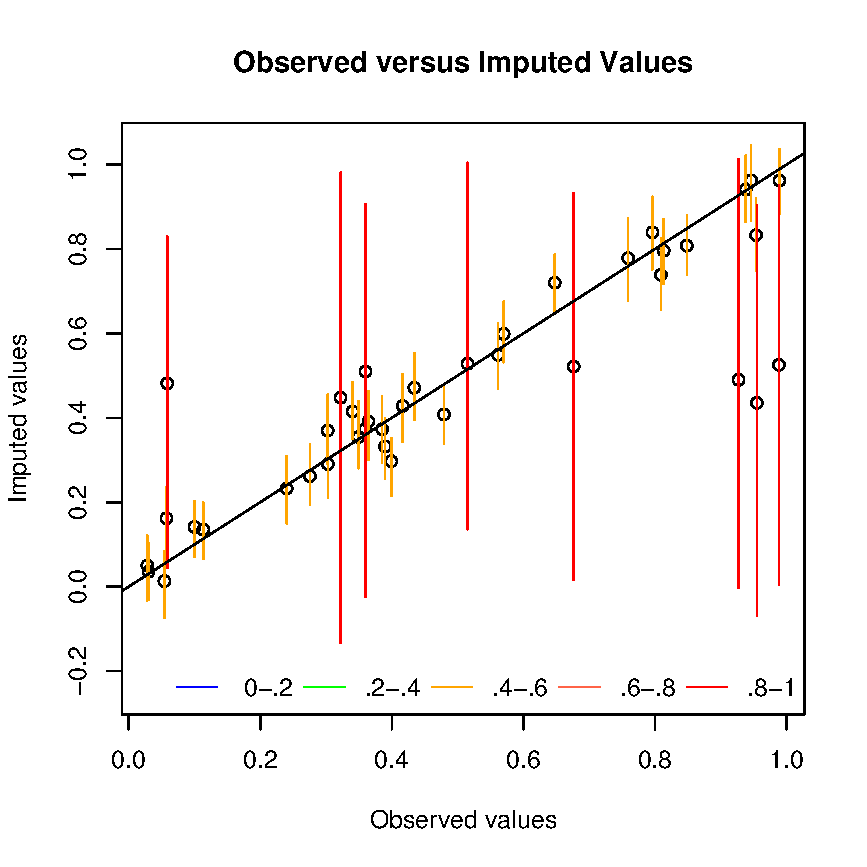
\includegraphics[scale=.8]{overimp}
  \caption{An example of the overimpute diagnostic graph.  Here
    ninety percent confidence intervals are constructed that detail
    where an observed value would have been imputed had it been
    missing from the dataset, given the imputation model.  The dots
    represent the mean imputation.  Around ninety percent of these
    confidence intervals contain the $y=x$ line, which means that the
    true observed value falls within this range.  The color of the
    line (as coded in the legend) represents the fraction of missing

    observations in the pattern of missingness for that observation.
    The yellow lines have more information (observed covariates) from
    which to impute the variable, and thus much tighter bounds.}
  \label{f:oi}
\end{figure}
Occasionally, the overimputation can display unintuitive results.  For
example, different observations may have different numbers of observed
covariates.  If covariates that are useful to the prediction are
themselves missing, then the confidence interval for this observation
will be much larger.  In the extreme, there may be observations where
the observed value we are trying to overimpute is \emph{the only}
observed value in that observation, and thus there is nothing left to
impute that observation with when we pretend that it is missing, other
than the mean and variance of that variable.  In these cases, we
should correctly expect the confidence interval to be very large.

An example of this graph is shown in figure \ref{f:oi}.  In this
simulated bivariate dataset, one variable is overimputed and the
results displayed.  The second variable is either observed, in which
case the confidence intervals are very small and the imputations
(yellow) are very accurate, or the second variable is missing in which
case this variable is being imputed simply from the mean and variance
parameters, and the imputations (red) have a very large and
encompassing spread.  The circles represent the mean of all the
imputations for that value.  As the amount of missing information in a
particular pattern of missingness increases, we expect the width of
the confidence interval to increase.  The color of the confidence
interval reflects the percent of covariates observed in that pattern
of missingness, as reflected in the legend at the bottom.

This graph can also be called from $R$ as:
\begin{verbatim}
 > output<-amelia(data=x) 
 > overimpute(data=x,output=output,var=3)
\end{verbatim}
where \texttt{var} is the column number (or the name) of the variable
you would like to produce the graph for.


\subsection{Overdispersed Starting Values}
\label{sec:overdisperse}

If the data given to \Amelia has a poorly behaved likelihood, the EM
algorithm can have problems finding a global maximum of the likelihood
surface and starting values can begin to effect imputations.  Because
the EM algorithm is deterministic, the point in the parameter space
where you start it can impact where it ends, though this is irrelevant
when the likelihood has only one mode.  However, if the starting
values of an EM chain are close to a local maximum, the algorithm may
find this maximum, unaware that there is a global maximum farther
away.  To make sure that our imputations do not depend on our starting
values, a good test is to run the EM algorithm from multiple,
dispersed starting values and check their convergence.  In a well
behaved likelihood, we will see all of these chains converging to the
same value, and reasonably conclude that this is the likely global
maximum.  On the other hand, we might see our EM chain converging to
multiple locations.  The algorithm may also wander around portions of
the parameter space that are not fully identified, such as a ridge of
equal likelihood, as would happen for example, if the same variable

were accidentally included in the imputation model twice.

\Amelia includes a diagnostic to run the EM chain from multiple
starting values that are overdispersed from the estimated maximum.
The overdispersion diagnostic will display a graph of the paths of
each chain.  Since these chains move through spaces that are in an
extremely high number of dimensions and can not be graphically
displayed, the diagnostic reduces the dimensionality of the EM paths
by showing the paths relative to the largest principle components of
the final mode(s) that are reached.  Users can choose between graphing
the movement over the two largest principal components, or more simply
the largest dimension with time (iteration number) on the $x$-axis.
The number of EM chains can also be adjusted.  Once the diagnostic
draws the graph, the user can visually inspect the results to check
that all chains convergence to the same point.
\begin{figure}[ht]\label{f:overgood}
  \centering 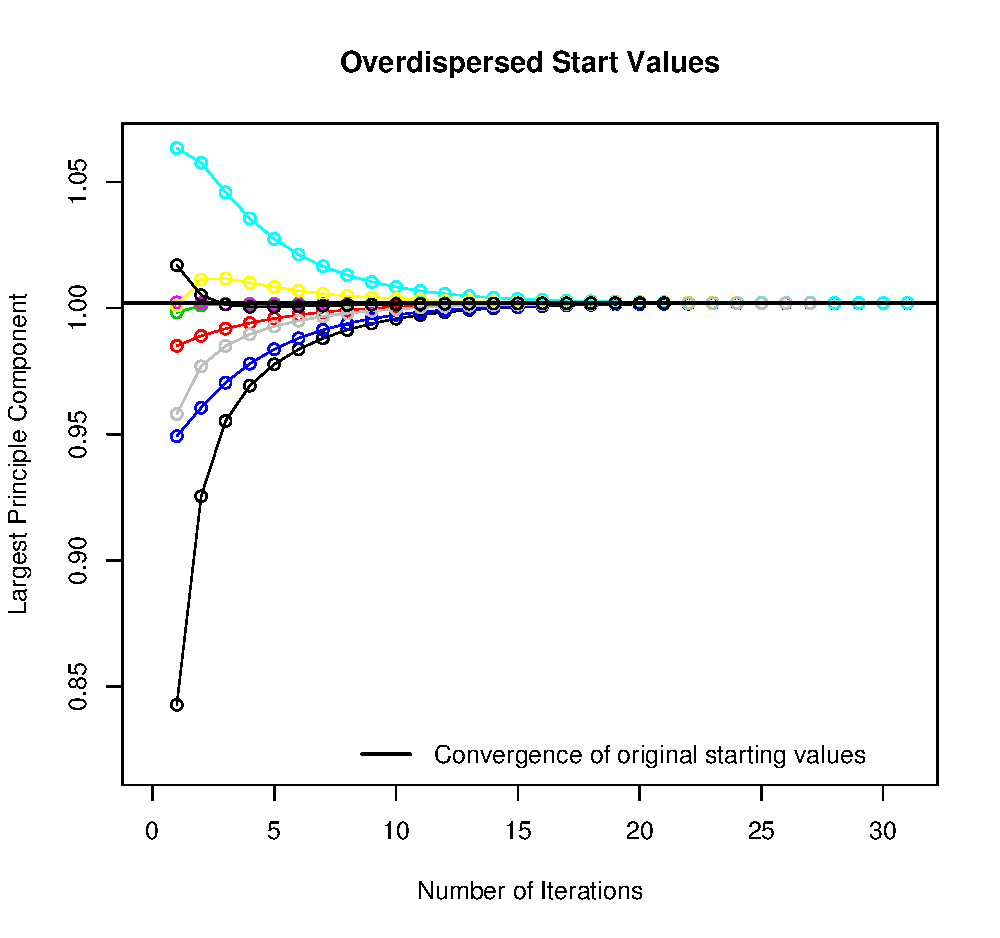
\includegraphics[scale=.7]{overdis1d}
  \caption{A plot from the overdispersion diagnostic where all EM
    chains are converging to the same mode, regardless of starting
    value.  The $y$-axis represents movement in the (very high
    dimensional) parameter space, and the $x$-axis represents the
    iteration number of the chain.}
\end{figure}

In one dimension, the diagnostic plots movement of the chain on the
$y$-axis and time, in the form of the iteration number, on the
$x$-axis.  Figures \ref{f:overgood} and \ref{f:overbad} show two examples of one dimensional plots.
The first shows a well behaved likelihood, as the starting values all
converge to the same point.  The black horizontal line is the point
where \Amelia converges when it uses the default method for choosing
the starting values.  The diagnostic takes the end point of this chain
as the possible maximum and disperses the starting values away from it
to see if the chain will ever finish at another mode.  Figure \ref{f:overbad} shows
an example of how a diagnostic plot will look on a problematic
likelihood surface.  A few of the iterations are ending up in vastly
different location in the parameter space.  This can happen for a
variety of reasons.  In this example it is a result of having two
highly collinear variables included in the imputation model.  More
generally, an unidentified imputation model will lead to non-unique ML
estimates (see King (1989) for a more detailed discussion of
identification and likelihoods).
\begin{figure}\label{f:overbad}
  \centering 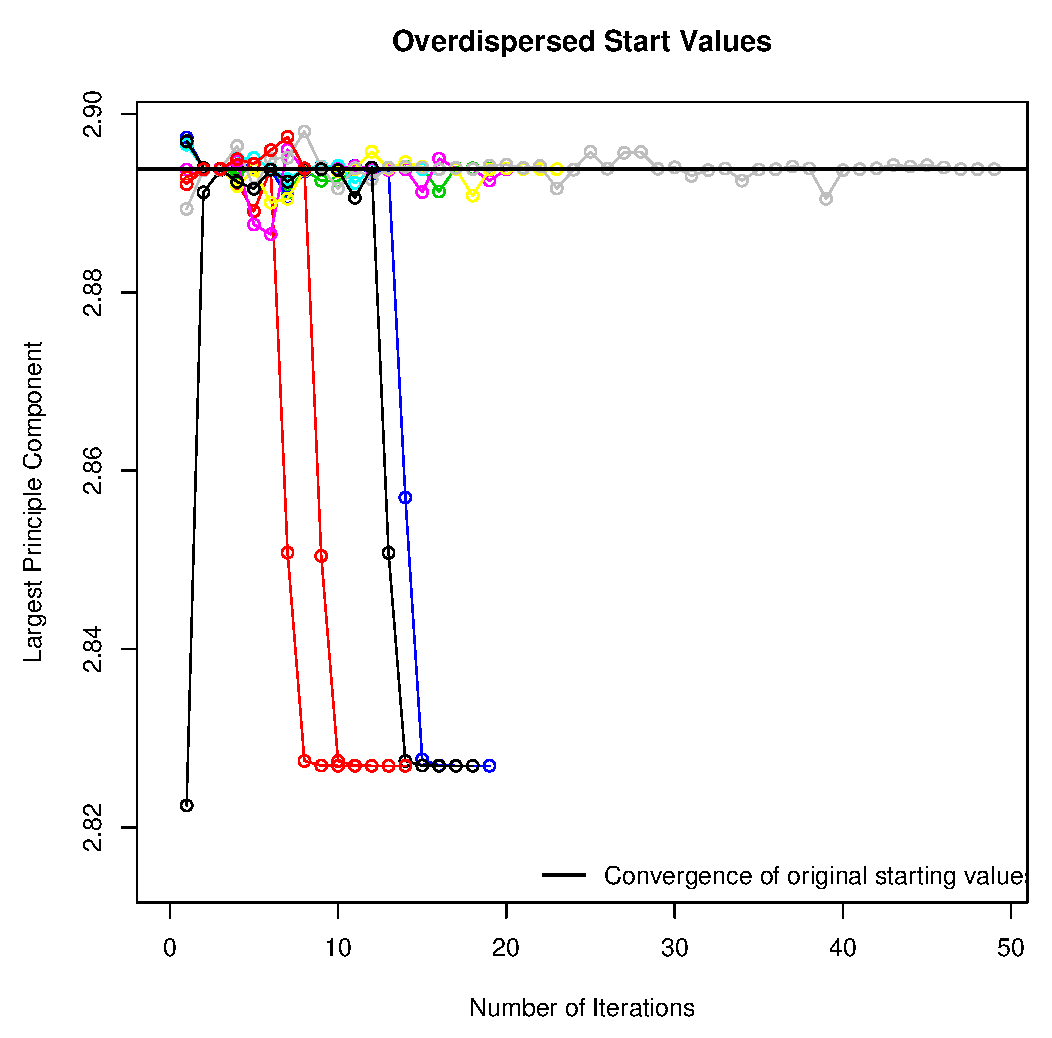
\includegraphics[scale=.5]{disperse-bad}
  \caption{ A problematic plot from the overdispersion diagnostic
    showing that EM chains are converging to one of two different
    modes, depending upon the starting value of the chain.}
\end{figure}

This graph can also be called from $R$ as:
\begin{verbatim}
 > output<-amelia(data=x) 
 > disperse(data=x,output=output,m=5,dims=1)
\end{verbatim}
where \texttt{dims} can be set to a value of either 1 (default) or 2,
for one dimensional and two dimensional graphs, respectively.  The
argument $m$ sets the number of EM chains to run to create the graph.
In $R$ this routine can also be called before an amelia run has taken
place, in which case output need not be declared, but any other amelia
options may be set in the same way they would be declared for the
amelia function.  This allows you to check the likelihood surface
\emph{before} running the amelia function.
\begin{figure}
  \centering 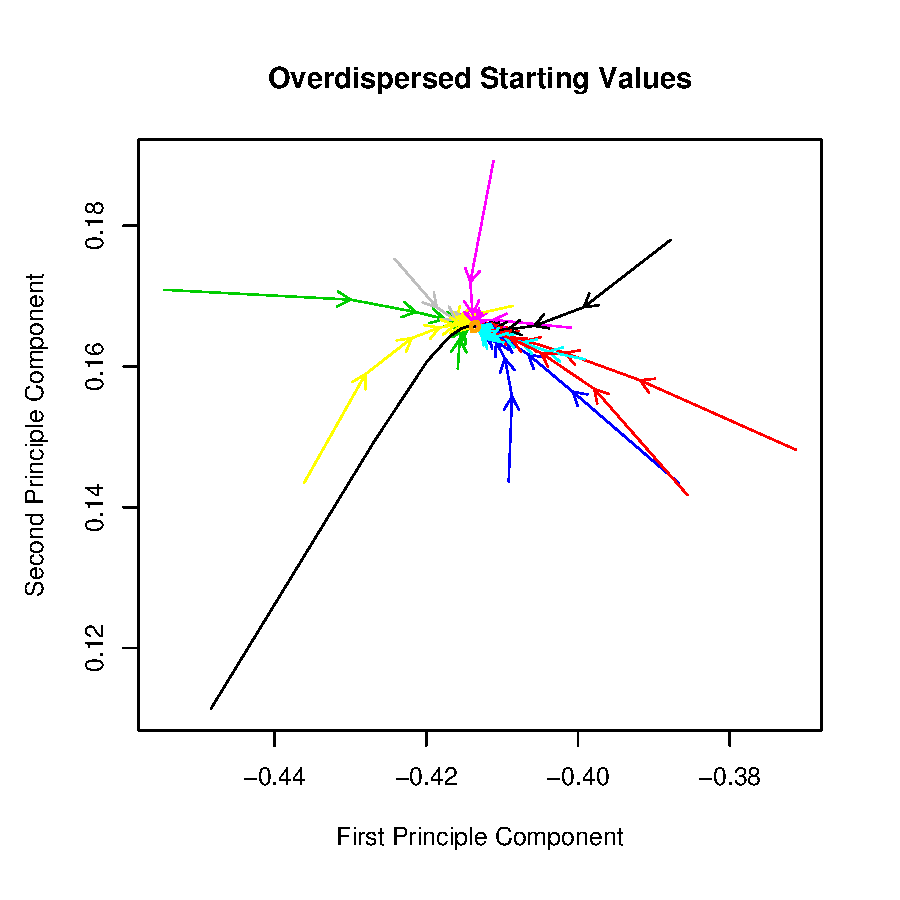
\includegraphics[scale=.7]{overdis2d}
  \caption{ A alternate way to visualize the plot visualizing the
    parameter space in two dimensions using the first two principal
    components of the end points of the EM chains.  The iteration
    number is no longer represented on the $y$-axis, although the
    distance between iterations is marked by the distance between
    arrowheads on each chain.}
\end{figure}

\section{Sessions}
\label{sec:sessions}

Setting options for some large datasets may take some time, especially
with the presence of many observational priors and non-linear
variables.  To ease this process, Amelia has the ability to save and
load sessions.  A saved session includes all options set by the user
in addition to any output information from Amelia.  Sessions are
useful for setting large numbers of options over multiple instances of
Amelia or imputing the data multiple times with the same setup.

In AmeliaView, you can save a session by opening the ``File'' menu and
selecting ``Save Session.''  This will open a dialog that will ask for
a filename (the file extenstion must be ``.r'').  To load a saved
session, simply navigate to the "File" menu and select "Load Session"
and locate the saved session file.  Note that the data file referenced
in the session file must be located in the same directory and have the
same name when attempting to load the session.  Upon loading, Amelia
configures all options to same values as the saved session.

In some cases you may wish to load a AmeliaView session at the R
command line.  To do so, use the \texttt{source} command to load the
session file which will add a list named \texttt{amelia.list} to your
working environment.  You can use this list in the \texttt{arglist}
options for the \texttt{amelia} function, which takes an Amelia output
or session list as its argument.  An example of loading a session at

the command line would be:

\begin{verbatim}
> source("am-session.R") 
> amelia.out <- amelia(data=x,arglist=amelia.list)
\end{verbatim}

In this example \texttt{am-session.R} is the session file and
\texttt{x} is the dataset that corresponds to the session file.  At
the command line, you must load the data into R seperately as sessions
are not tied to specific datasets at the command line.  When provided
to Amelia, the argument list will take precendence over other
arguments.  For example, specifying an identification variable with
\texttt{idvars} while also using \texttt{arglist} will result in
Amelia ignoring the \texttt{idvars} provided by the user and refer to
the idvars setting in \texttt{arglist}.

\section{AmeliaView Menu Guide}
\label{sec:menu}

\subsection{Step 1 - Input}
\label{sec:step1}
\begin{figure}[ht]
 \begin{htmlonly} 
  \centering 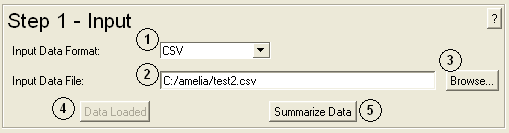
\includegraphics[scale=1]{step1} 
 \end{htmlonly}
 \begin{latexonly}
  \centering 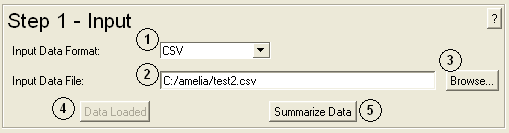
\includegraphics[scale=.75]{step1}
 \end{latexonly}
  \caption{Detail for step 1 on the front page of AmeliaView.}
\end{figure}
\begin{enumerate}
\item \textbf{Input Data Format} - Pick the format for your dataset.
  The format you pick will be the default format that is shown when
  you open the ``Browse'' dialog.  Currently, ${\mathfrak Amelia}$
  supports five different file formats: Comma-Separated Values (.CSV),
  Tab-Delimited Text (.TXT), Stata v.5-8 (.DTA), SPSS (.DAT), and SAS
  Transport (.XPORT).
\item \textbf{Input Data File} - Enter the location of your dataset.
  If your file is located in a high level directory, it might be
  you are trying to access for more information.
\item \textbf{Summarize Data} - View plots and summary statistics for
  the individual variables.  This button will bring up a dialog box
  with a list of variables.  Clicking on each variable will display
  the summary statistics on the right.  Below these statistics, there
  is a ``Plot Variable'' button, which will show a histogram of the
  variable.  For data that are string or character based, AmeliaView
  will not show summary statistics or plot histograms.
\end{enumerate}


\subsection{Step 2 - Options}

\label{sec:step2}
\begin{figure}[ht]
 \begin{htmlonly} 
  \centering 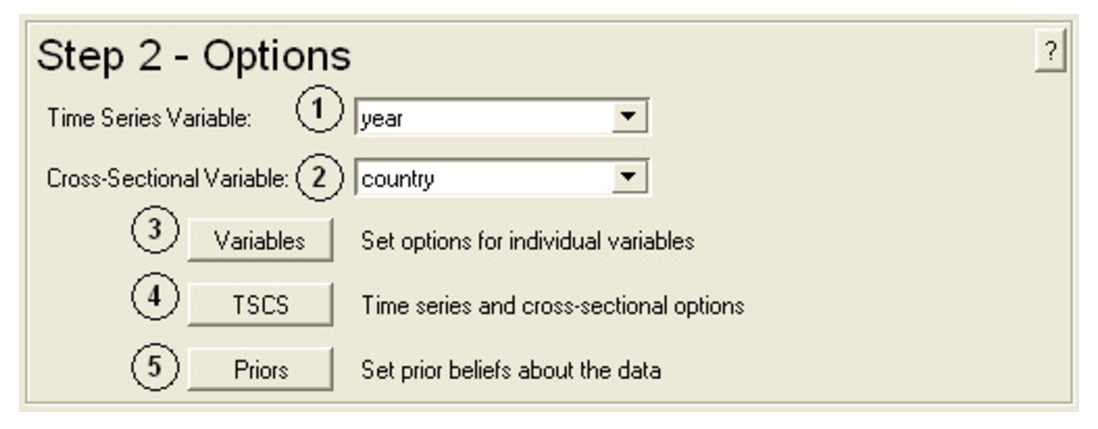
\includegraphics[scale=1]{step2} 
 \end{htmlonly}
 \begin{latexonly}
  \centering 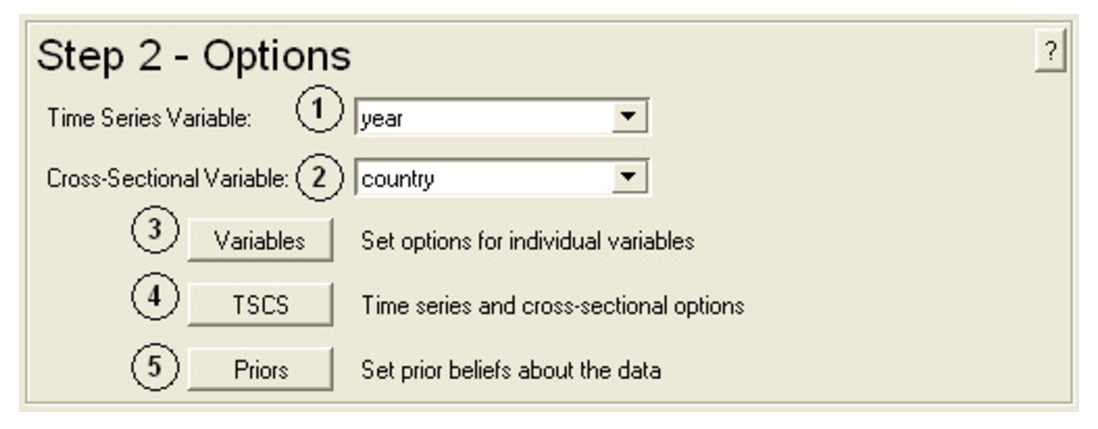
\includegraphics[scale=.75]{step2}
 \end{latexonly}
  \caption{Detail for step 2 on the front page of AmeliaView.}
\end{figure}
\begin{enumerate}
\item \textbf{Time Series Variable} - Choose the variable that indexes
  time in the dataset.  If there is no time series component in your
  data, set it to ``(none).''  You must set this option in order to
  access the Time Series Cross Sectional options dialog.
\item \textbf{Cross Sectional Variable} - Choose the variable that
  indexes the cross-section.  You must set this in order to access the
  ``Set Case Priors'' in the ``Priors'' dialog.
\item \textbf{Variables} - Becomes available after you load the data.
  See \ref{sec:vardiag} for more information.
\item \textbf{TSCS} - Becomes available after you set the Time Series
  variable.  See \ref{sec:tscsdiag} for more information.
\item \textbf{Priors} - Becomes available after you load the data.
  See \ref{sec:pridiag} for more information.
\end{enumerate}

\subsubsection{Variables Dialog}
\label{sec:vardiag}
\begin{figure}[ht]
 \begin{htmlonly} 
  \centering 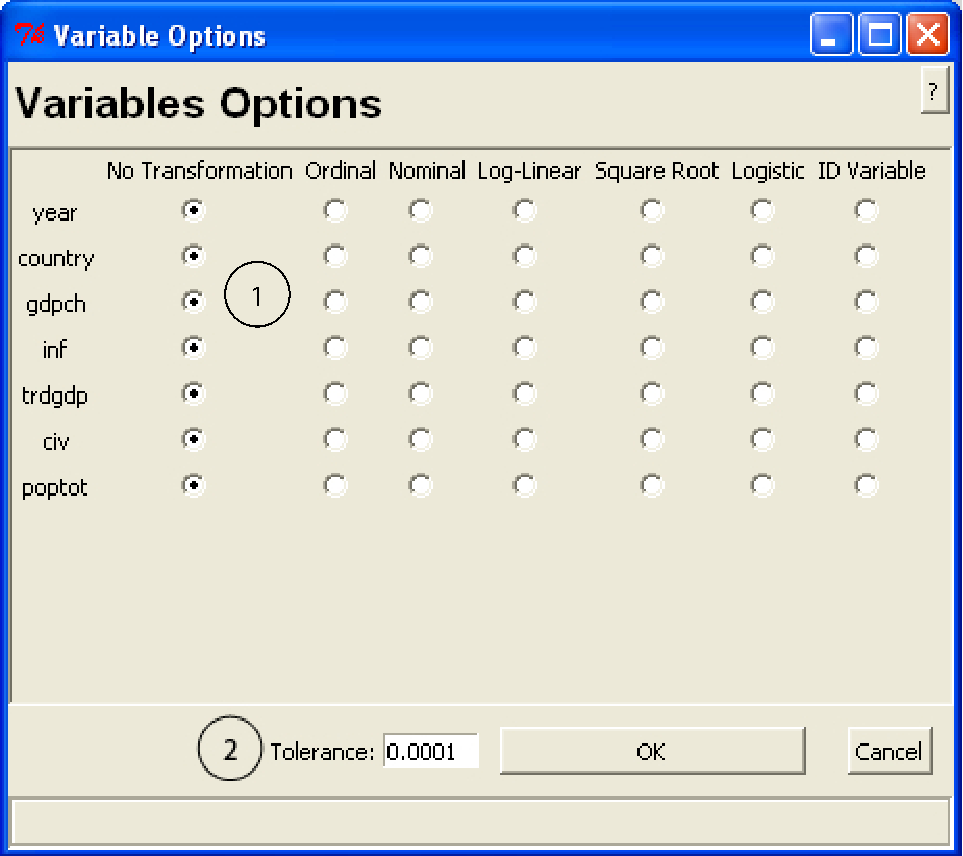
\includegraphics[scale=1]{varopts} 
 \end{htmlonly}
 \begin{latexonly}
  \centering 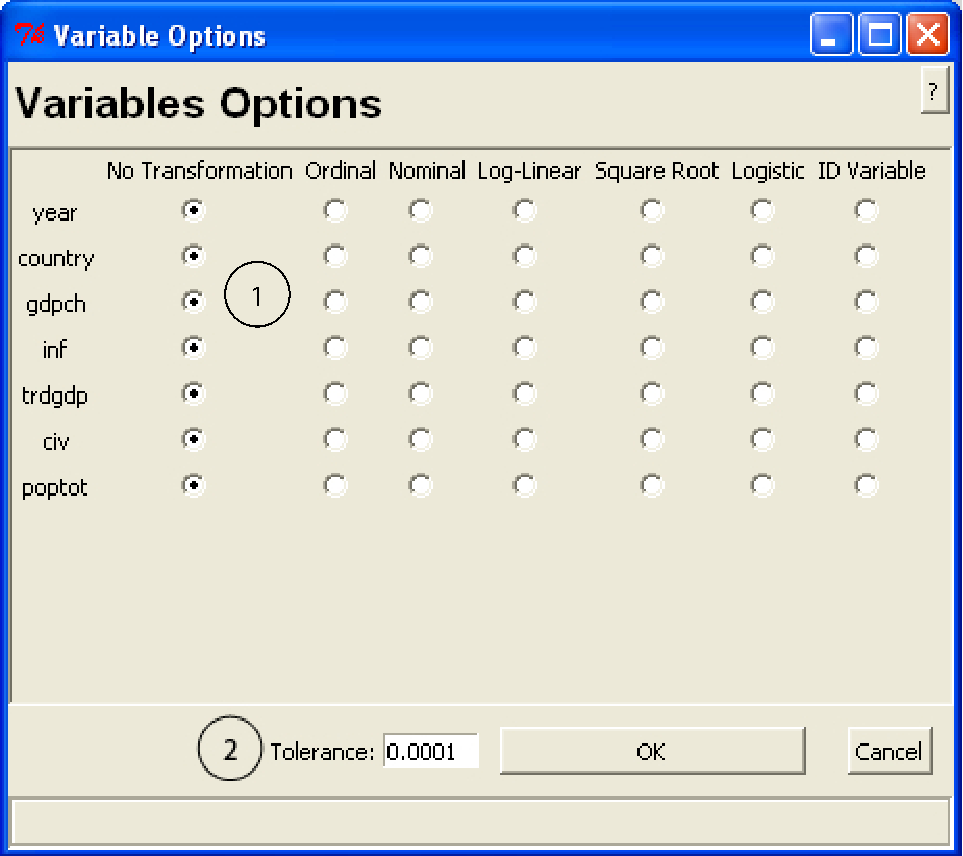
\includegraphics[scale=.75]{varopts}
 \end{latexonly}
  \caption{Detail for Variable Options dialog.}
\end{figure}
\begin{enumerate}
\item \textbf{Variable Transformations} - Choose the transformation
  that best normalizes for the variable, if any exists.  See
  \ref{sec:trans} on Transformations to see how each transformation is
  useful.  You can also choose whether or not the variable is an ID
  variable.  If so, it will be left out of the imputation model, but
  will remain in the dataset.  This is useful for variables that have
  no explanatory power like extra case identifiers.
\item \textbf{Tolerance} - Adjust the level of tolerance that \Amelia
  uses to check convergence of the EM algorithm.  If you imputations
  seem to never converge, increasing this value will speed up convergence.
\end{enumerate}


\subsubsection{Time Series Cross Sectional Dialog}
\label{sec:tscsdiag}
\begin{figure}[ht]
 \begin{htmlonly} 
  \centering 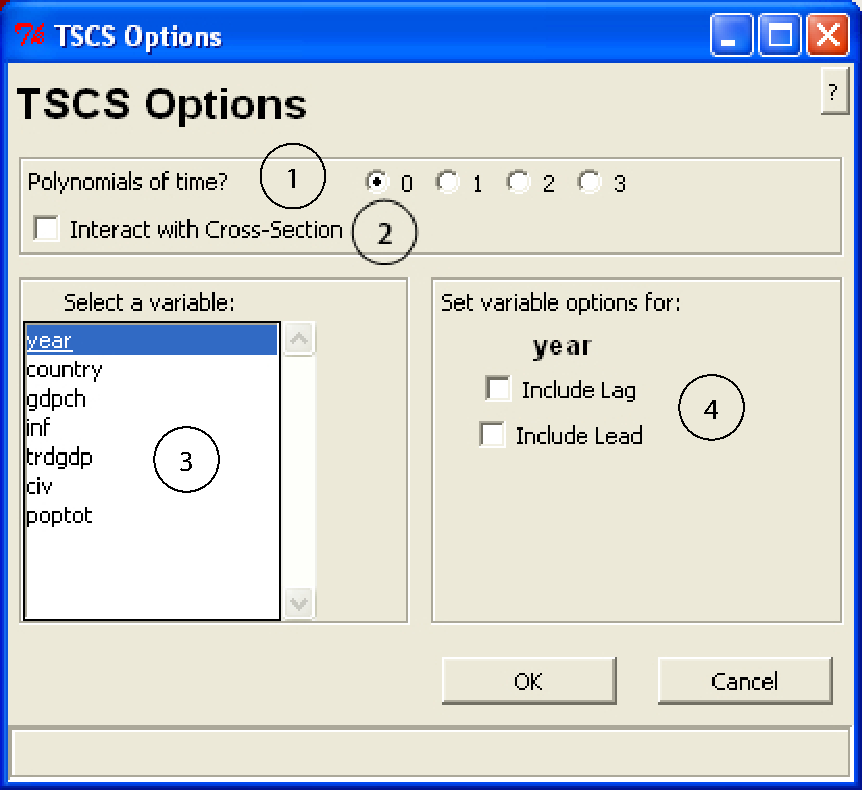
\includegraphics[scale=1]{tscs} 
 \end{htmlonly}
 \begin{latexonly}
  \centering 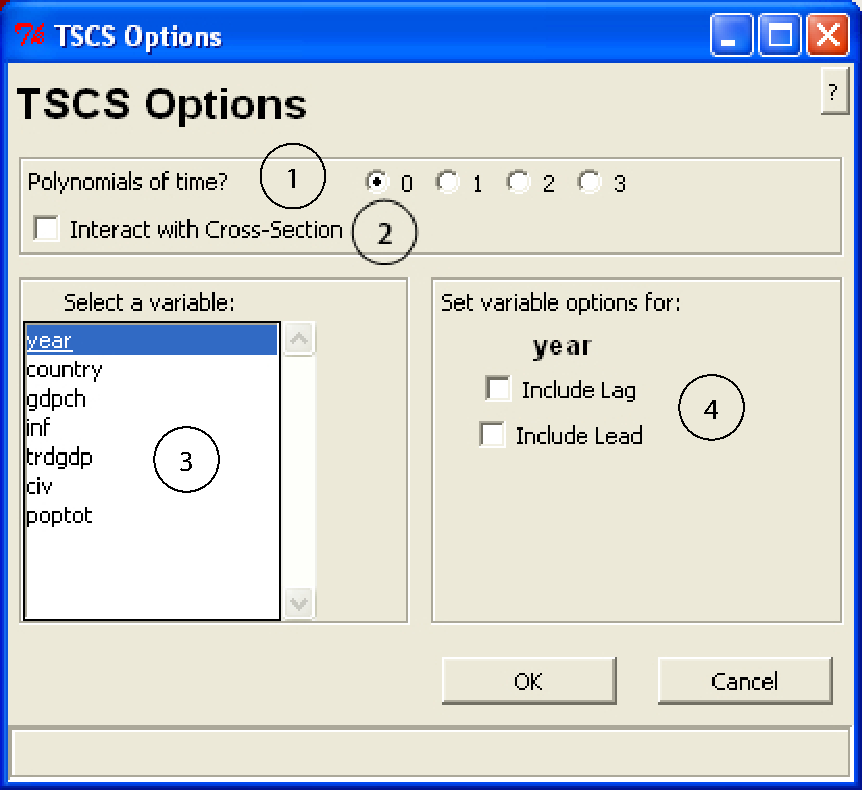
\includegraphics[scale=.75]{tscs}
 \end{latexonly}
  \caption{Detail for Time-Series-Cross-Section Options dialog.}
\end{figure}
\begin{enumerate}
\item \textbf{Polynomials of Time} - This option, if activated, will
  have ${\mathfrak Amelia}$ use trends of time as a additional
  condition for fitting the missing data.  The higher the level of
  polynomial will allow more variation in the trend structure, yet it
  will take more degrees of freedom to estimate.
\item \textbf{Interact with Cross-Section} - Interacting this with the
  cross section is way of allowing the trend of time to vary across
  cases as well.  Using a 0 level polynomial and interacting with the
  cross section is the equivalent of using a fixed effects.  For more
  information see \ref{sec:tscs} above.
\item \textbf{Variable Listbox} - Choose the variable whose lag you
  would like to set.
  condition for fitting the missing data.  The higher the level of
  polynomial will allow more variation in the trend structure, yet it
  will take more degrees of freedom to estimate.
\item \textbf{Interact with Cross-Section} - Interacting this with the
  cross section is way of allowing the trend of time to vary across
  cases as well.  Using a 0 level polynomial and interacting with the
  cross section is the equivalent of using a fixed effects.  For more
  information see \ref{sec:tscs} above.
\item \textbf{Variable Listbox} - Choose the variable whose lag you
  would like to set.
\item \textbf{Lag Settings} - Choose to include lags and leads in the
  data set to handle the effects of time.  See \ref{sec:tscs} above.
\end{enumerate}

\subsubsection{Priors Dialog}
\label{sec:pridiag}
\begin{figure}[ht]
 \begin{htmlonly} 
  \centering 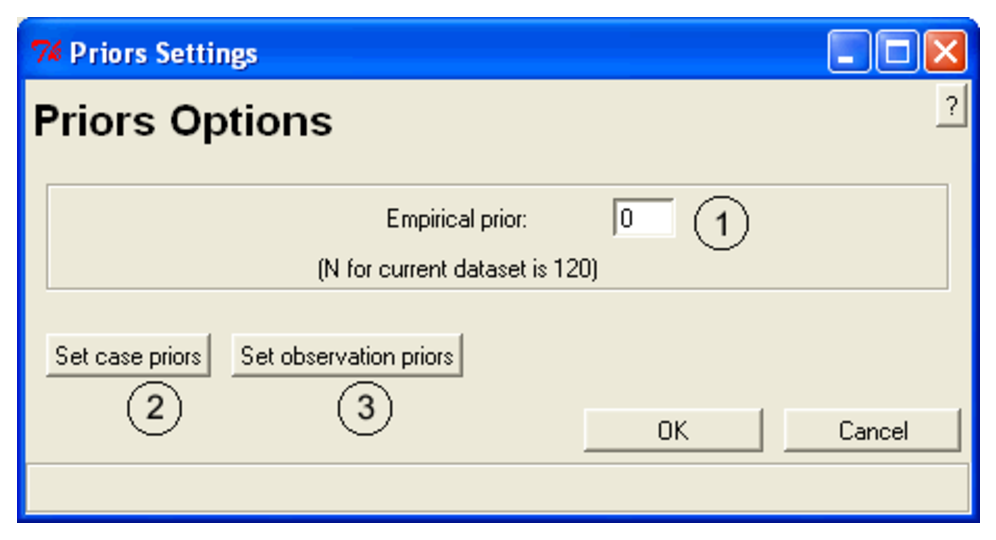
\includegraphics[scale=1]{priors} 
 \end{htmlonly}
 \begin{latexonly}
  \centering 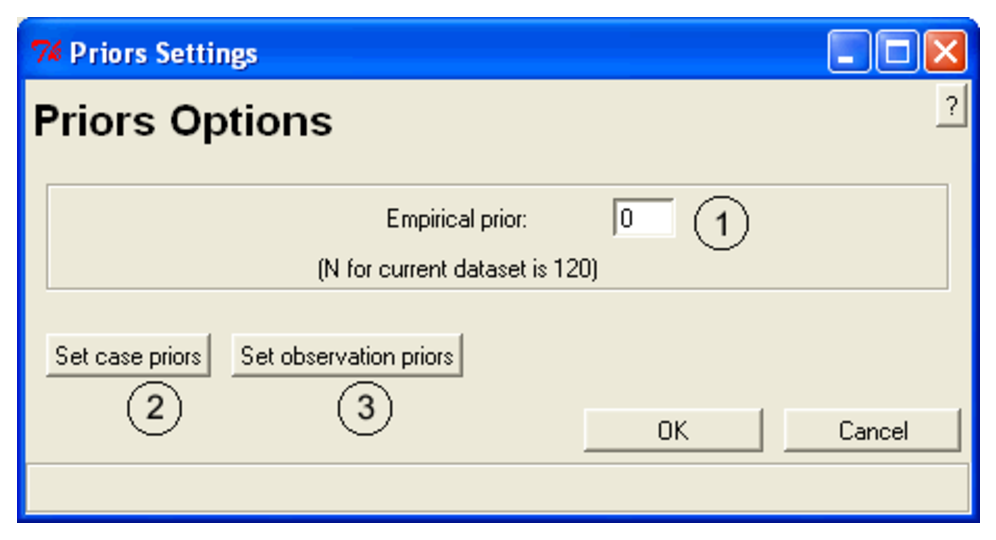
\includegraphics[scale=.75]{priors}
 \end{latexonly}
  \caption{Detail for Priors Options dialog.}
\end{figure}
\begin{enumerate}
\item \textbf{Empirical Prior} - A prior that adds observations to
  your data in order to shrink the covariances.  A useful place to
  start is around 5\% of the total observations in the dataset.
\item \textbf{Variable Listbox} - Select the variable for which you
  want to set a range prior.
\item \textbf{Range Prior} - If you
  have a prior belief about the range of possible values that a
  variable can take, enter the lower and upper bound.
\item \textbf{Set Case Priors} -
  Tell ${\mathfrak Amelia}$ which cases are similar.  See
  \ref{sec:casepri} for more details about case priors.
\item \textbf{Set Observational Priors} - Set prior beliefs about 
 ranges for individual missing observations.  For more information 
 about observational priors, see \ref{sec:obspri}.
\end{enumerate}

\subsubsection{Case Priors}
\label{sec:refcasepri}
\begin{figure}[ht]
 \begin{htmlonly} 
  \centering 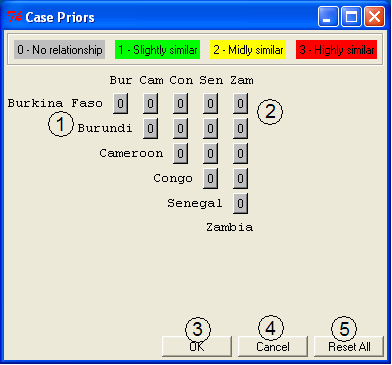
\includegraphics[scale=1]{case} 
 \end{htmlonly}
 \begin{latexonly}
  \centering 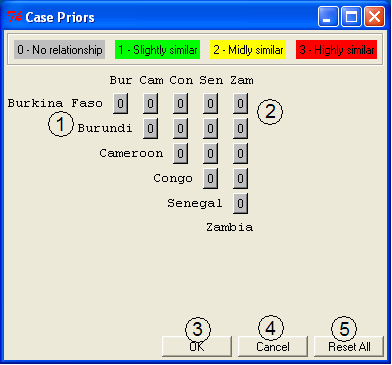
\includegraphics[scale=.75]{case}
 \end{latexonly}
\caption{Detail for Case Priors dialog.}
\end{figure}
\begin{enumerate}
\item \textbf{Case Names} - The row and column name for each button
  indicate the relationship that the button controls.  For instance,
  the top-left button in the ``Burkina Faso'' row and the ``Burundi''
  column; thus, the setting on this button will indicate the strength
  of the similarity prior between these two cross-sections.
\item \textbf{Buttons} - Toggling the buttons will change the setting
  for each case.  The higher the number on the button, the stronger
  the indicated relationship is believed to be.  Find the column of
  the first country and then follow it down to the row of the similar
  country.  Press the button to raise the level similarity from 0 to 1
  to 2 to 3.  You can reset the case priors by hitting the ``Reset
  All'' button in the top left corner.
\item \textbf{OK} - Close the window and save any changes.
\item \textbf{Cancel} - Close the window and discard any changes.
\item \textbf{Reset All} - Sets all case priors to the default 0
  setting.
\end{enumerate}

\subsubsection{Observational Priors}
\label{sec:refobspri}
\begin{figure}[h]
 \begin{htmlonly} 
  \centering 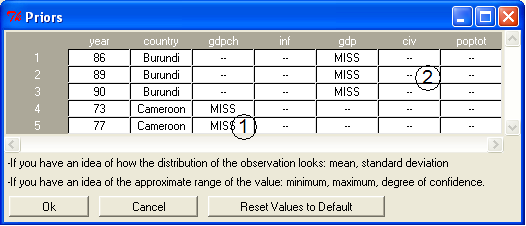
\includegraphics[scale=1]{obspri} 
 \end{htmlonly}
 \begin{latexonly}
  \centering 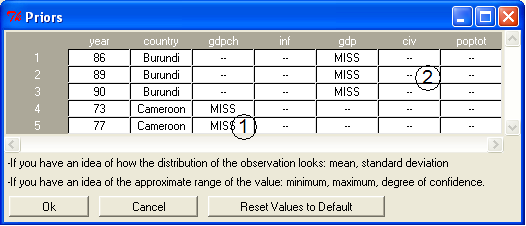
\includegraphics[scale=.75]{obspri}
 \end{latexonly}
\caption{Detail for Observational Priors dialog}
\end{figure}
\begin{enumerate}
\item \textbf{Missing Cell} - A missing value in the data.  Click on
  the cell to enter your prior beliefs about the value.  Enter your
  prior beliefs as a range of possible values as with a comma in
  between (e.g. \texttt{0,10000}).
\item \textbf{Observed Cell} - Non-missing values cannot be selected
  since there is no way to incorporate a prior about an observed
  value.
\end{enumerate}

\subsection{Step 3 - Output}
\label{sec:step3}


\begin{figure}[ht]
 \begin{htmlonly} 
  \centering 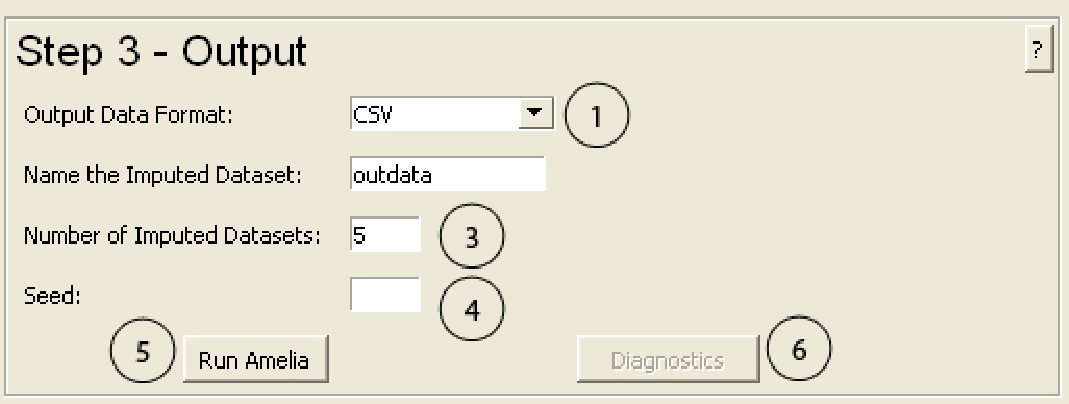
\includegraphics[scale=1]{step3} 
 \end{htmlonly}
 \begin{latexonly}
  \centering 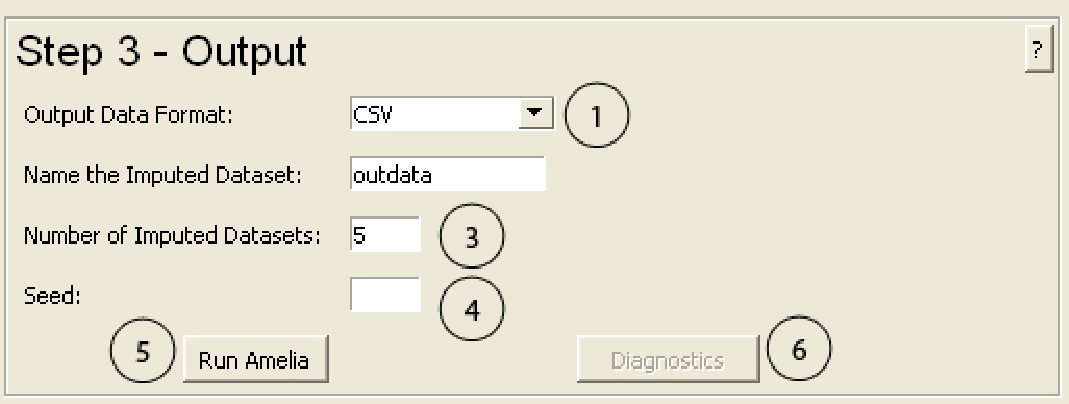
\includegraphics[scale=.75]{step3}
 \end{latexonly}
  \caption{Detail for step 3 on the front page of AmeliaView.}
\end{figure}
\begin{enumerate}
\item \textbf{Output Data Format} - Choose the format of output data.
  If you would like to not save any output data sets (if you wanted,
  for instance, to simply look at diagnostics), set this option to
  ``(no save).''  Currently, you can save the output data as: Comma
  Separated Values (.CSV), Tab Delimited Text (.TXT), or Stata (.DTA).
\item \textbf{Name of Imputed Datasets} - Enter the prefix for the
  output data files.  If you set this to ``mydata'', your output files
  will be \texttt{mydata1.csv, mydata2.csv...} etc.  Try to keep this
  name short as some operating systems have a difficult time reading
  long filenames.
\item \textbf{Number of Imputed Datasets} - Set the number of
  imputations you would like.  In most cases, 5 will be enough to make
  accurate predictions about the means and variances.
\item \textbf{Run Amelia} - Runs the ${\mathfrak Amelia}$ procedure on
  the input data.  A dialog will open marking the progress of
  ${\mathfrak Amelia}$.  Once it is finished, it will tell you that
  you can close the dialog.  If an error message appears, follow its
  instructions; this usually involves closing the dialog, resetting
  the options, and running the procedure again.
\item \textbf{Diagnostics} - Post-imputation diagnostics.  The only
  currently available graph compares the densities of the observed
  data to the mean imputation across the $m$ imputed datasets.
\end{enumerate}


\subsubsection{Diagnostics Dialog}
\label{sec:diagdiag}
\begin{figure}[ht]
 \begin{htmlonly} 
  \centering 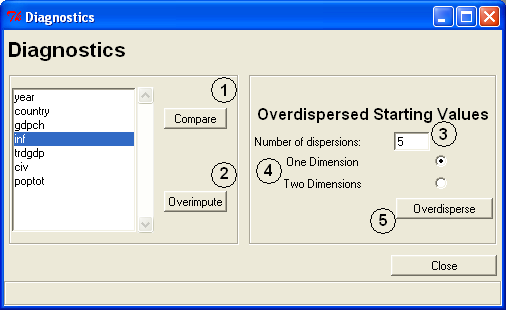
\includegraphics[scale=1]{diag} 
 \end{htmlonly}
 \begin{latexonly}
  \centering 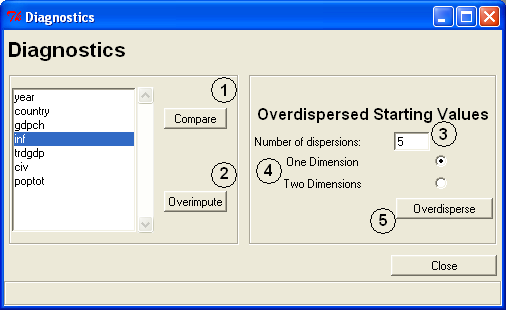
\includegraphics[scale=.75]{diag}
 \end{latexonly}
  \caption{Detail for Diagnostics dialog.}
\end{figure}
\begin{enumerate}
\item \textbf{Compare Plots} - This will display the relative
  densities of the observed (red) and imputed (black) data.  The
  density of the imputed values are the average imputations across all
  of the imputed datasets.
\item \textbf{Overimpute} - This will run \Amelia on the full data
  with one cell of the chosen variable artificially set to missing and
  then check the result of that imputation against the truth.  The
  resulting plot will plot average imputations against true values
  along with 90\% confidence intervals.  These are plotted over a
  $y=x$ line for visual inspection of the imputation model.
\item \textbf{Number of overdispersions} - When running the
  overdispersion diagnostic, you need to run the imputation algorithm
  from several overdispersed starting points in order to get a clear
  idea of how the chain are converging.  Enter the number of
  imputations here.
\item \textbf{Number of dimensions} - The overdispersion diagnostic
  must reduce the dimensionality of the paths of the imputation
  algorithm to either one or two dimensions due to graphical
  restraints.
\item \textbf{Overdisperse} - Run overdispersion diagnostic to
  visually inspect the convergence of the \Amelia algorithm from
  multiple start values that are drawn randomly.
\end{enumerate}

\bibliographystyle{apsr}
\bibsep=0in
\bibliography{gk.bib,gkpubs.bib}
\end{document}

